\documentclass[twoside, a4paper, fleqn, reqno]{article}
\usepackage[
	assignmentNumber=4, 
	authorZero={Stijn Kammer},
	studentNumberZero={4986296},	
	authorOne={Ramon Kits},
	studentNumberOne={5440769},
	groupNumber={31}
]{reportStyle}


\begin{document}

\maketitle

\section*{Exercise 1}
\begin{enumerate}
	\item\textbf{Consider a CRC that uses the divisor 10011. Find two collisions with
	10101011, that is, find two other data values that produce the same
	CRC checksum as 10101011.}
	\\First we have to compute the CRC checksum of \texttt{10101011} using the divisor \texttt{10011}.
	\\\texttt{\phantom{}10101011\color{red}0000}
	\\\texttt{\phantom{}\underline{10011~~}~~~~~}
	\\\texttt{\phantom{}~~11001~~~~~}
	\\\texttt{\phantom{}~~\underline{10011~}~~~~}
	\\\texttt{\phantom{}~~~10101~~~~}
	\\\texttt{\phantom{}~~~\underline{10011~~}~~}
	\\\texttt{\phantom{}~~~~~110\color{red}00~~}
	\\\texttt{\phantom{}~~~~~\underline{100\color{red}11~}~}
	\\\texttt{\phantom{}~~~~~~10\color{red}110~}
	\\\texttt{\phantom{}~~~~~~\underline{10\color{red}011~}}
	\\\texttt{\phantom{}~~~~~~~~\color{red}1010}
	\\The CRC checksum is therefore 1010.
	Now we have to find two other data values that produce the same CRC checksum.
	The first place where zeros have been added has to be the same in order to
	find a collision. In this case, we have to find a value that produces a 
	step where \texttt{110\color{red}00} is used. That is, the first step where
	CRC bits are being added. So to make it easy to find a collision,
	we can just use \texttt{110} as value because this generates the step we need instantly.
	Also, we can use one of the other intermediate steps to find a collision, e.g. \texttt{10101}.
	This way of finding collisions is very limited, only steps of the original value can be used.
	To find a collision with a value of the same length as the original, we can also
	use the divisor as the first part of the value so when a XOR is performed on that part,
	the first 5 bits will get discarded in a sense.
	At this point, we are left with 3 bits that have to be \texttt{110} to get the desired step we want.
	So the value we end up with is \texttt{10011110}.\\
	We now have found three collisions using two different methods.
	Collisions can also be found in more sophisticated ways, but with the simplicity of the question
	in mind, only two ways are discussed here. Our found values are
	\textbf{\underline{\texttt{110}}}, \textbf{\underline{\texttt{10101}}} and \textbf{\underline{\texttt{10011110}}}.
	Which are more than two, but it makes it possible to demonstrate multiple ways of finding collisions.
	

	\item\textbf{Consider a CRC that uses the divisor 10011. Suppose the data value
	is 11010110. Trudy wants to change the data to 111*****, where "*"
	indicates that she doesn't care about the bit in that position, and she
	wants the resulting checksum to be the same as for the original data.
	Determine all data values Trudy could choose.}
	For this question, we have to find all data values that Trudy could choose.
	Now we cannot use the same method as in the previous question because we want 
	all possible data values that start with \texttt{111} and have a length of 8 bits.
	Trudy has the opportunity to generate any of $2^5=32$ possible values for the remaining 5 bits,
	of which only a select amount create the same CRC checksum as the original data value.
	Brute forcing all options is possible but not scalable. So we have to find a way to
	compute the possible values without having to check all of them.	
	\\We have to solve for the unknown bits in the following checksum calculation steps.
	\\\texttt{\phantom{}111*****\color{red}0000}
	\\\texttt{\phantom{}\underline{10011~~}~~~~~}
	\\\texttt{\phantom{}~11...~~~~~~~~}
	\\\texttt{\phantom{}~\underline{10011}~~~~~~~~}
	\\\texttt{\phantom{}~~1...~~~~~~~}
	\\\texttt{\phantom{}~~\underline{10011}~~~~~~}
	\\\texttt{\phantom{}~~~...~~~~~~}
	\\\texttt{\phantom{}~~~\underline{...~~}~~~~}
	\\\texttt{\phantom{}~~~~~110\color{red}00~~}
	\\\texttt{\phantom{}~~~~~\underline{100\color{red}11~}~}
	\\\texttt{\phantom{}~~~~~~10\color{red}110~}
	\\\texttt{\phantom{}~~~~~~\underline{10\color{red}011~}}
	\\\texttt{\phantom{}~~~~~~~~\color{red}1010}
	\\For the one step before we reach \texttt{110\color{red}00}, we can say that there are a small
	group of possibilities for the unknown bits.
	\\We can fill in the empty step in the only possible way, and we can remove that step all together.
	That gives us the two only solutions.
	\\Filling these values in the checksum calculation steps, we get the following results.
	\\\texttt{\phantom{}11100111\color{red}0000~~~}					\texttt{\phantom{}~~~~~11110100\color{red}0000}
	\\\texttt{\phantom{}\underline{10011~~}~~~~~~~~}				\texttt{\phantom{}~~~~~\underline{10011~~}~~~~~}
	\\\texttt{\phantom{}~11111~~~~~~~~~}							\texttt{\phantom{}~~~~~~11011~~~~~~~~}
	\\\texttt{\phantom{}~\underline{10011}~~~~~~~~~}				\texttt{\phantom{}~~~~~~\underline{10011}~~~~~~~~}
	\\\texttt{\phantom{}~~11001~~~~~~~~}							\texttt{\phantom{}~~~~~~~10000~~~~~~}
	\\\texttt{\phantom{}~~\underline{10011}~~~~~~~~}				\texttt{\phantom{}and~~~~\underline{10011}~~~~~~}
	\\\texttt{\phantom{}~~~10101~~~~~~~}							\texttt{\phantom{}~~~~~~~~~~110\color{red}00~~}
	\\\texttt{\phantom{}~~~\underline{10011}~~~~~~~}				\texttt{\phantom{}~~~~~~~~~~\underline{100\color{red}11~}~}
	\\\texttt{\phantom{}~~~~~110\color{red}00~~~~~}					\texttt{\phantom{}~~~~~~~~~~~10\color{red}110~}
	\\\texttt{\phantom{}~~~~~\underline{100\color{red}11~}~~~~}		\texttt{\phantom{}~~~~~~~~~~~\underline{10\color{red}011~}}
	\\\texttt{\phantom{}~~~~~~10\color{red}110~~~~}					\texttt{\phantom{}~~~~~~~~~~~~~\color{red}1010}
	\\\texttt{\phantom{}~~~~~~\underline{10\color{red}011~}~~~}		
	\\\texttt{\phantom{}~~~~~~~~\color{red}1010~~~}					
	\\The only two answers are \textbf{\underline{\texttt{11100111}}} and \textbf{\underline{\texttt{11110100}}}. 

\end{enumerate}

\section*{Exercise 2}

Code for this exercise can be found at Themis.

\section*{Exercise 3}

Code for this exercise can be found at Themis.

\section*{Exercise 4}

To compute this probability, the best way to approach this is by calculating The
probability of everyone having a distinct fingerprint and subtracting that from 1.
But how do we calculate that probability?\\
We can take the product of the probabilities of each person getting a distinct fingerprint.
This can be calculated using the following formula:
\begin{equation}
	\label{eq:1}
	P_{distinct}(t, p)=\prod_{n=1}^{p} \frac{t+1-n}{t}
\end{equation}
Where $t$ is the number of possible fingerprints and $p$ is the number of people.
This equation can be simplified to:
\begin{equation}
	\label{eq:2}
	P_{distinct}(t, p)=\frac{\frac{t!}{(t-p)!}}{t^p}
\end{equation}
If we put in the values $t=2^{160}$ and $p=7.5\times10^{9}$, it becomes apparent the simplified
equation is not very helpful. It has to calculate $(2^{160})^{7.5\times10^{9}}$, which is an unimaginably large number.
No computer can calculate this number. Therefore, we have to use the original equation.
Code can be written to calculate this probability, calculations have pointed out this will take
around 25 minutes to complete.\\
Doing this with a basic script would however not work. For these types of calculations we need
high precision floating point numbers. Python does not have these by default. Computers in general
cannot easily compute with high precision floating point numbers needed for this calculation.
If we want to calculate this probability, we need to use a library that can handle these numbers.
But doing this makes the calculation take significantly longer. So long that it is not feasible to
calculate this probability this way. And even then, the code would most likely output a wrong
answer due to the physical limitations of computers. We have to approximate the probability.

Let us take a look at equation \ref{eq:1} again. Since $p \ll t$, and also $p^{2} \ll t$, we can approximate the product function
by using the following approximation:
\begin{equation}
	\label{eq:3}
	P_{collision}(t, p) \approx \frac{p^{2}}{2t}
\end{equation}
This equation is not fully accurate, but it is accurate enough for this problem.
Filling in the values $t=2^{160}$ and $p=7.5\times10^{9}$, we get:
\begin{equation}
	\label{eq:4}
	P_{collision}(t, p) \approx \frac{(7.5\times10^{9})^{2}}{2\times2^{160}} \approx 2\times10^{-29}
\end{equation}
This is a very small probability. This shows that getting a hash collision is highly unlikely.
This probability is negligible as of today.\\

% \begin{equation}
% 	\label{eq:5}
% 	(1 - x)^{p} \geq (1 - p \times x)~for~0 \leq x \leq 1
% \end{equation}

\section*{Exercise 5}

\begin{enumerate}
	\item The conflict of interest classes are:
	\begin{enumerate}
		\item \{$C_1$, $C_3$\}
		\item \{$C_2$, $C_4$, $C_6$\}
		\item \{$C_5$\}
	\end{enumerate}
	These classes share the same interests. The first class shares the interests of the finance sector,
	the second class shares the interests of the pharmaceutical sector and the third class shares the
	interests of the media sector.\\
	\item The diagram for the conflict of interest classes is:
	\begin{figure}[H]
		\centering
		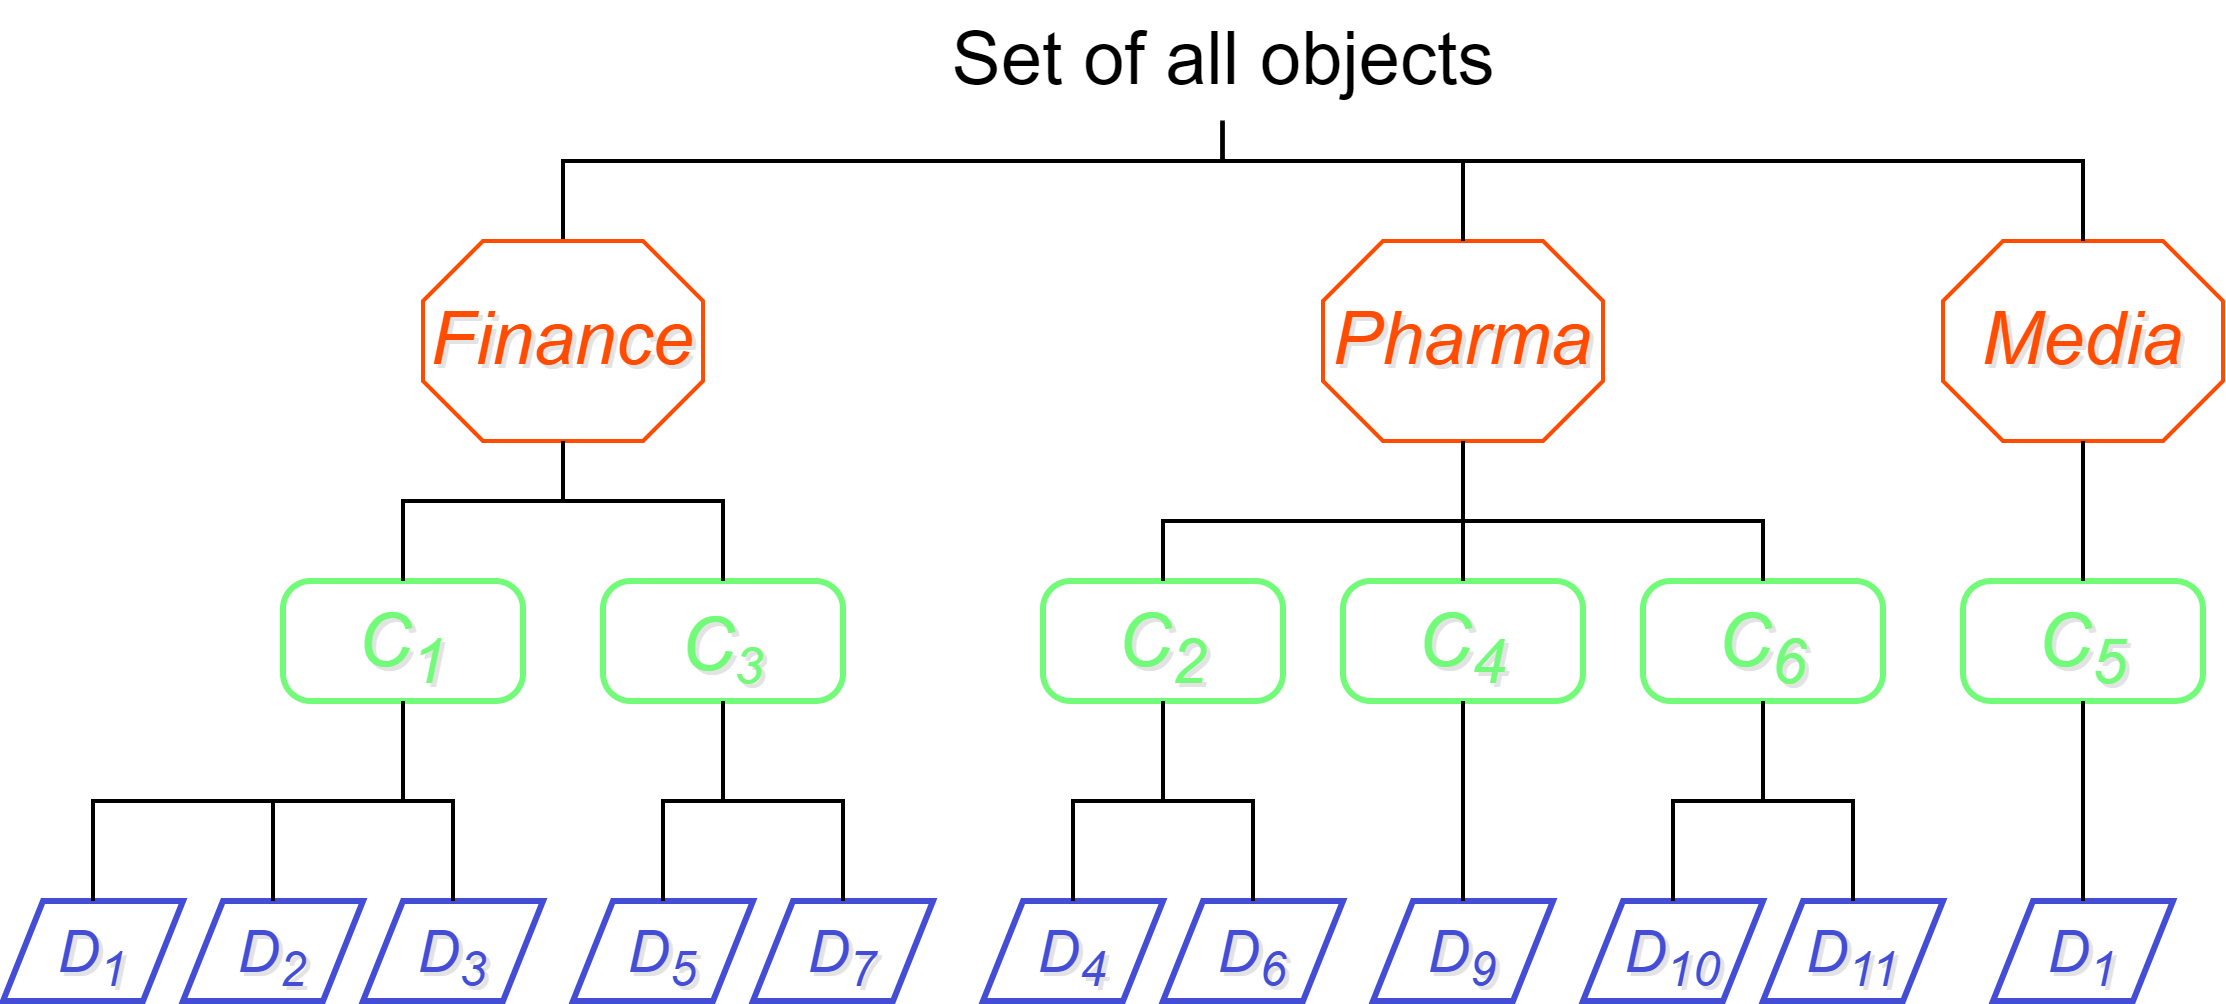
\includegraphics[width=0.8\textwidth]{./media/chinese_wall_policy.drawio.png}
		\caption{Conflict of interest classes, with the Chinese wall policy.}
	\end{figure}
	Where the orange octagons represent the conflict of interest classes,
	the green rounded rectangles represent the clients and the blue parallelograms represent the documents.

\end{enumerate}

\section*{Exercise 6}

\begin{enumerate}
	\item This policy targets subjects with the role named \texttt{Manager} and the
	resource named \texttt{Report1}. If both values are given but one or more of these conditions is not met, e.g. the role \texttt{Employee} is given,
	the policy will consider target to be "No Match". If previous situations do not apply and one or more values are not given,
	the policy will consider the target to be "Indeterminate" because both of the values must be present.\\
	When the target is a match, the two rules are checked. The first rule checks whether access should
	be denied. This first rule has two conditions. The first condition checks for the subject client.
	If for this condition the value "C" is given, this specific condition is met and will return true.
	The second condition checks whether the resource is confidential or not. If this value is not given, the
	condition will assume the resource is not confidential. If the resource is confidential, the condition will return true.
	When both conditions returned true, the first rule will return an access decision of "Deny".
	The second rule will return an access decision of "Permit" no matter what.\\
	Since this policy has a \texttt{deny-overrides rule-combining} algorithm, the deny decision has priority over the permit decision.
	Therefore, the second rule will only apply if the first rule does not apply.\\

	In short, the policy will deny access to the resource \texttt{Report1} for the subject with the role \texttt{Manager} if the subject client
	is given as "C" and the resource is confidential, otherwise it will grant access. If the subject role is not \texttt{Manager}, or the resource is not \texttt{Report1},
	the policy will not grant or deny access to any resource.\\
	
	\item First of all, the values \texttt{subject(division, Finance)} and \texttt{action(action-id, read)} are not used by the policy,
	so there is no need discussing those values. When the target is checked, both values are given and both conditions are met. The subject
	role is \texttt{Manager} and the resource ID is \texttt{Report1}.\\
	The client value is not given, however when this is not given, the policy assumes the client is not "C". The resource is confidential because
	\texttt{resource(confidential, true)}, but since the client is not "C", access is not getting denied. The second rule will return an access decision of "Permit" and that also will
	be the final access decision.\\
\end{enumerate}

\section*{Exercise 7}

Kerberos ensures that the authentication is completed within the authentication's allowed lifespan
by saving the timestamp of the authentication. The timestamp is saved in the Ticket Granting Ticket (TGT).
This ticket is also sent to the client. The client can use this ticket to request a service ticket from the
Kerberos server. The Kerberos server will check the timestamp of the TGT. If the timestamp is still valid,
the Kerberos server will grant the service ticket. If the timestamp is not valid, the Kerberos server will
deny the service ticket.
The Ticket Granting Ticket is encrypted with the Ticket Granting Service's (TGS) secret key. This ensures
that the client cannot change the timestamp of the TGT.

The client receives the TGT with the encrypted timestamp because one of the goals of Kerberos is to
be stateless. This is what makes Kerberos so scalable. The Kerberos server does not need to keep track
of the authentication's timestamp. The client can keep track of this information that way.

\section*{Exercise 8}

\begin{enumerate}
	\item SSL does not imply authentication. When using SSL, the client and server can authenticate each other.
	However, the server does not need to authenticate the client. To do proper authentication, the client
	needs to send a certificate to the server. The server can then check the certificate to see if it is valid.
	\item The meaning of "doing authentication" is that the client and server are sure that they are communicating
	with the correct party. This is done by using a certificate. The certificate is signed by a trusted authority.
	\item \textit{https://www.icce.rug.nl} is properly authenticated because the certificate is verified by a trusted authority.
	The certificate is issued by "GEANT Vereniging" and the final certificate authority is "AAA Certification Services".
	\item The certificate of \textit{https://www.icce.rug.nl} is issued on 2022-01-20 and will expire on 2023-01-21.
\end{enumerate}

\section*{Exercise 9}

\begin{enumerate}
	\item The k-anoymity level is the minimal number of records that have all the quasi-identifiers in common.
	In this case, there are 3 variations of quasi-identifier records. Hispanics of age 18,
	Afro-Americans of age 34 and Caucasians of age 21.
	These records occur 3, 3 and 2 times respectively. The minimum
	number of records that contain the same quasi-identifiers is therefore 2. Meaning that the k-anoymity level
	is \textbf{\underline{2}}.\\
	\item The table contains 3 classes. Every class contains only records with identical quasi-identifiers.
	Every class contains only one type of disease, the sensitive attribute. So every record
	in a class has the same sensitive attribute. Therefore, the l-diversity level is 1.
	This is not a good level of diversity. The l-diversity level should be as high as possible without
	losing too much information. This is because the higher the l-diversity level, the more unsure
	you can be about the sensitive attribute.

	Knowing every record of a class has the same attributes and there are only 3 classes.
	The only way in which the l-diversity level can be higher than 1 is by removing all quasi-identifiers.
	So even though the l-diversity level is 1, it is not feasible to try to increase it.
	
\end{enumerate}

\section*{Exercise 10}

\end{document}